\def\pathToRoot{.}
\documentclass[a4paper, 12pt]{article}

\usepackage[utf8]{inputenc}
\usepackage{ifthen}
\usepackage{xparse}
\usepackage{scrextend}
\usepackage{setspace}
\usepackage{verbatim}
\usepackage{color}
\usepackage[inline]{enumitem}
\usepackage[colorlinks=true, linkcolor=black, citecolor=black]{hyperref}

\usepackage{tikz}
\usepackage{pgfplots}
\usepackage{bbold}
\usepackage{listings}

\usepackage{subcaption}

\usepackage{amsmath}
\usepackage{amssymb}
\usepackage{latexsym}
\usepackage{hyperref}
\usepackage{cleveref}

\definecolor{gray}{rgb}{0.2,0.2,0.2}

\pagenumbering{arabic}


\usepackage[a4paper, left=2cm, top=2cm, right=2cm, bottom=2cm]{geometry}

\usepackage{multirow}
\usepackage{fancyvrb}

\newcommand{\vect}[1]{\boldsymbol{#1}}

\newcounter{exerciseCounter}
\setcounter{exerciseCounter}{0}

\newcommand{\exerciseNumber}{\sheetnumber.\arabic{exerciseCounter}}

\setenumerate{label=\alph*)}

% Sheet Header
\newcommand{\exercisehead}[3]
{
    \def\sheetnumber{#1}
    \begin{center}
        \begin{minipage}{0.45\linewidth}
            \textsc{Universität des Saarlandes}
            \par
           Prof. Dr. Dietrich  Klakow
           \par
           Lehrstuhl für Signalverarbeitung
           \par
           NNIA Winter Term 2019/2020
        \end{minipage}
        \begin{minipage}{0.45\linewidth}
            \begin{flushright}
               
\includegraphics[width=0.30\linewidth]{headers/lsv_logo.jpg}
            \end{flushright}
        \end{minipage}
        \vspace{5pt}
        \hrule
        \vspace{12pt}
        \doublespacing
        {
            \LARGE
            \textbf{Exercise Sheet #1}
        }
        \par
        {
            \large
            #2
        }
        \par
        \ifdefined\issolution
        \textit{(Solutions)}
        \else
        \fi
        
    \textbf{Deadline: #3}

    \end{center}
    \vspace{2pt}
    \hrule
    \vspace{12pt}
}

% Exercise environment
\NewDocumentEnvironment{exercise}{oo}
{
	\refstepcounter{exerciseCounter}
	\par
	\vspace{12pt}
    \noindent
    \textbf{Exercise \exerciseNumber \  - #1}\IfNoValueF{#2}{\hfill(#2 points)}
	\vspace{12pt}
	\par
	\begin{addmargin}[12pt]{0pt}
}
{
    
	\end{addmargin}
	\par
	\vspace{12pt}
}

% Solution environment
\newenvironment{solution}
{
		\ifthenelse{\isundefined{\issolution}}
		{
			\comment
		}
		{
			\par
			\color{gray}
			\vspace{6pt}
			\textit{Solution \exerciseNumber}
			\par
			\begin{addmargin}[30pt]{0pt}
		}
}
{
		\ifthenelse{\isundefined{\issolution}}
		{
		}
		{
			\end{addmargin}
			\par
			\vspace{12pt}
		}
}



\usepackage{cleveref}

\def\issolution{}

\begin{document}

% {Sheet number}{headline}{deadline}
\exercisehead{10}{\small Philip Georgis [s8phgeor], Pauline Sander [s8pasand], Vilém Zouhar [vizo00001] }{02.02.2021}

\section*{Exercises}

\newcommand{\TODO}[1]{\textcolor{red}{TODO:#1}}

\begin{exercise}[Architecture][0.5 + 1.5 = 2]

\begin{enumerate}
	\item What is the benefit of an LSTM over RNN? Give a short explanation (2-4 sentences).
	\item Draw an LSTM cell and provide the formulas used to calculate each element. Explain
the function of each element.  
\end{enumerate}

\end{exercise}


\begin{solution}
    \begin{enumerate}
        \item LSTM contains explicit input, output and forget gates. It alleviates the vanishing gradient problem. Furthermore, an LSTM is better at handling long-distance dependencies as the memory state always contains some information on previous states.
        \item \Cref{fig:lstm_schema} shows an LSTM cell. It processes the input as follows:
        \begin{enumerate}
            \item[1.] $e_t = concat(x_t,c_{t-1})$ The LSTM cell takes an input $x_t$, the $t^{th}$ element of the sequence, as well as the control state $c_{t-1}$ of the previous LSTM cell (same as previous output) and concatenates them. 
            \item[2.] The LSTM cell also takes the memory state $m_{t-1}$ of the previous LSTM cell.
            \item[3.] $f_t = sigm(W_f\times e_t + b_f)$ contains values [0,1] and is based on $e_t$. The forget gate removes (reduces the intensity of) parts of the memory state through element wise multiplication with $f_t$: $g_t = f_t * m_{t-1}$
            \item[4.] $h_t = sigm(W_h\times e_t + b_h)$ works in a way similar to $g_t$. $i_t = h_t * tanh(W_i \times e_t + b_i)$ is the information contained in $e_t$ that should be added to the memory state.
            \item[5.] $m_t = i_t + g_t$ is the new memory state.
            \item[6.] Parts of this new memory become the new control state (removing information the same way as in step 4): $c_t = j_t * tanh(W_c \times e_t + b_c)$ with $j_t = sigm(W_j\times e_t + b_j)$
            \item[7.] $o_t$ is the output at position t, identical to $c_t$.
            \item[8.] The new memory and control states $m_t$ and $c_t$ are passed on to the next cell.
        \end{enumerate}
        \begin{figure} [h]
            \centering
            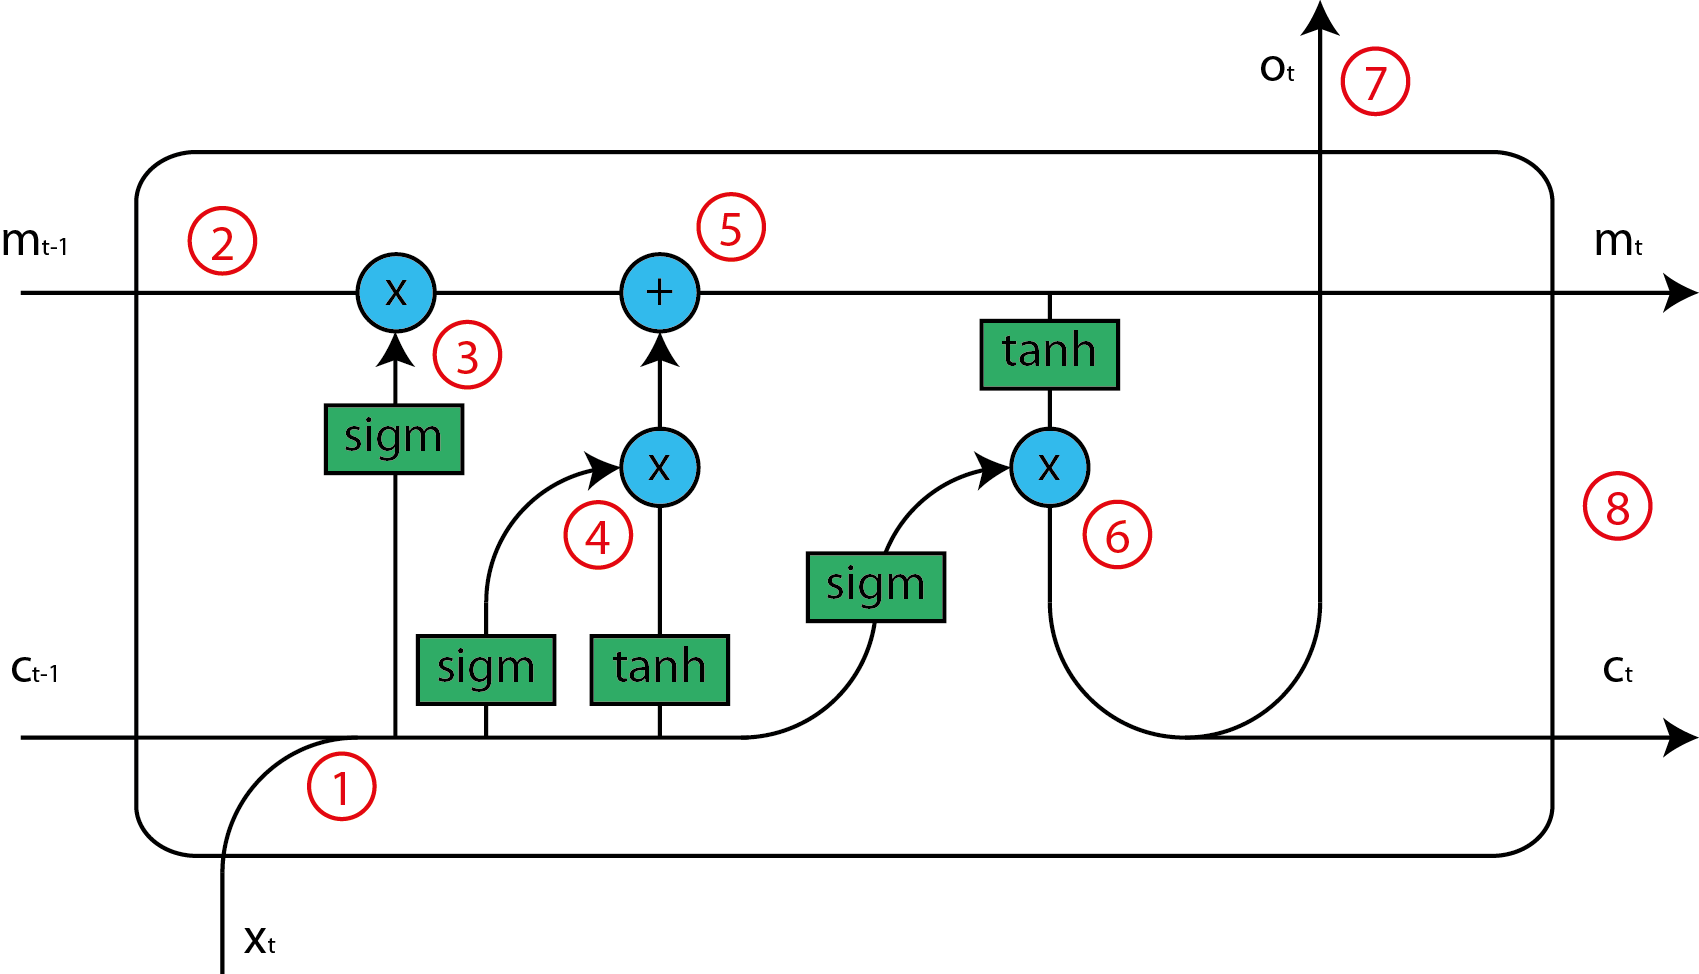
\includegraphics{img/LSTM.png}
            \caption{LSTM schema}
            \label{fig:lstm_schema}
        \end{figure}
    \end{enumerate}
\end{solution}

\begin{exercise}[Embeddings] [1 + 0.5 + 0.5 = 2]

    To perform the following exercise you have to read an \href{https://towardsdatascience.com/from-pre-trained-word-embeddings-to-pre-trained-language-models-focus-on-bert-343815627598}{article about static and contextualized embeddings.} Answer the following questions based on the article:

    \begin{enumerate}
        \item Give short explanations of static and contextualized word embeddings. Provide examples.
        \item What are the advantages of contextualized (dynamic) word embeddings over static ones?
        \item What is transfer learning? On which task is a model (e.g. BERT) pre-trained? (\textbf{Hint:} read the article till the end) Can we pre-train without any task? Why / why not?
    \end{enumerate}
        
\end{exercise}

\begin{solution}
    \begin{enumerate}
    \item Static embeddings (e.g. word2vec) produce one vector given a single word or subword unit. This is an issue for homographs: \textit{man} is going to have the same word embedding for both the noun and the verb.
    
    Contextualized word embeddings (e.g. BERT) produce the vector representation given a single word and also the current context. The word \textit{man} would have different embeddings in the sentences \textit{\textbf{Man}, is it cold today?} and \textit{Go \textbf{man} the post!} and \textit{He is a \textbf{man} of few words.}
    
    \item The issue with homographs is not the primary driver for contextualized word embeddings. The primary advantage of contextualized/dynamic word embeddings is that they better enable us to capture more meaning of the word. A disadvantage would be that the resulting model is much bigger.
    
    \item In transfer learning the model is trained on one task, but then the task changes. The model can be slightly modified to suit the new task, e.g. by substituting the top layer so that the shape fits, etc. BERT is trained on masked language modeling and next sentence prediction (technically \textit{Does the second sentence follow from the first one?}).
    \end{enumerate}
    
    For the pre-training we do still need some rudimentary task to be defined, so that the model can be optimized with respect to some defined loss.
\end{solution}

\begin{exercise}[Exam Preparation][6]

Start preparing for the exam: \\
Go over all the chapters and create the structure of the course.
You can do it in form of a mind map, bullet points structure etc., whatever format works better for you.

\end{exercise}


\begin{solution}
    Numbers corresponds to chapters according to the slides.
    \begin{enumerate}[label=\hspace{-0.8cm}\textbf{Ch. \arabic*}, align=left]
        \item Organization.
        \item Showcasing NN input architectures (image classification, ASR, MT); language model definition.
        \item Basic linear algebra concepts; Eigendecomposition; SVD; PCA
        \item The general task of ML; capacity; cross-validation; MLE; SVM (briefly); linear regression
        \item Feed-forward NN; gradient-based optimization (esp. gradient descent); learning rate; Jacobian ($\rightarrow \mathbb{R}^n$) \& Hessian ($\rightarrow \mathbb{R}$, second order) matrix; Newton method (second order optimization); Taylor series; activation functions (ReLU, TanH, sigmoid); loss functions (MSE, cross-entropy)
        \item Chain-rule; computational graphs; multilayer perceptron; universal approximation
        \item Regularization (esp. norm penalties); data augmentation; multitask learning; early stopping; parameter sharing/tying; bagging/ensemble methods; dropout; adversarial training
        \item Optimization algorithms; stochastic/batch/minibatch GD; ill-conditioning; plateaus; local minima; cliffs and vanishing/exploding gradients; SGD, SGD with momentum, AdaGrad, RMSProp, Adam (+bias correction); parameter initialization; pre-training
        \item Mathematical convolution; 2D convolution; convolutional layer (receptive field, parameter sharing, multi-channel input); pooling (max, avg); hyperparameters (kernel size, padding and stride); structured output
        \item RNNs and their computation graphs; RNN training/inference; sequence modelling and connected tasks; biRNN; seq2seq (encoder-decoder); recursive NNs; long-term dependencies; LSTM; explicit memory; Transformer (RNN-less encoder, decoder still sequential); attention
    \end{enumerate}
\end{solution}


\end{document}
